\chapter{Reading a report, step by step}\label{ch:walkthrough}

This chapter follows real samples through the commissioned chain, from the file that goes in to the report that comes out. Every number
quoted here is printed in the report the chain wrote for that sample, and every report was made by the one command a researcher runs after
downloading the repository: no step was done by hand. The three reports are kept with their bundles in the repository
(Biological\_Physics/MethylPhys/doors/data/REPORT\_EXAMPLES\_V4/final). The showcase runs add their reports here as each is read.

\section{One command}

A researcher who has cloned the repository and installed the chain's requirements reads an array with
\begin{center}\small\texttt{python3 run\_sample.py --grn <Grn.idat> --red <Red.idat> --specimen "whole blood" --ref-table <refs.csv> --out sample.html}\end{center}
and a sequencing sample, aligned with Bismark, with
\begin{center}\small\texttt{python3 run\_sample.py --bam <sample.bam> --ref-fasta <genome.fa> --out sample.html}\end{center}
The reference table is optional; it names healthy samples run on the same day, and when it is given Met-A and the C-score are tared against them,
so that the laboratory's own habits cancel out (Chapter~\ref{ch:chain}). Each run writes one HTML page with two views, a Researcher view that opens
first and a Plain view, the same report as two PDFs, the run's bundle as JSON, and one row in the evidence ledger (Chapter~\ref{ch:report}).

\section{A healthy whole-blood array}

The first sample is a healthy whole-blood array from a public study (GEO series GSE235717, sample GSM7508429), Illumina EPIC v1, read against three
healthy arrays from the same study as its same-run references. It is one of the arrays on which the C-score's healthy band was set, so no unread
data was spent on it.

\paragraph{Intake.} Stage~0 checks the file before anything is read: both color channels are present and unchanged (their checksums are recorded),
99.9\,\% of probes are detected, 99.8\,\% have at least three beads, and the call rate is 99.75\,\%. The chain predicts the donor's sex from the X and Y
probes (female) and, because none was declared, records that it could not compare. Verdict: proceed.

\paragraph{Whose cells.} The IAM-Deconvolver reads the cell shares against IAM-Atlas v2.1: neutrophils 46.6\,\% (95\,\% interval 43.3--50.1),
CD4 T cells 23.3\,\%, CD8 T cells 10.2\,\%, monocytes 6.3\,\%, NK cells 8.1\,\% and B cells 5.7\,\%. The first four are commissioned; the report
prints the B and NK shares with the line \emph{This share is preliminary until the IAM-Deconvolver is officially commissioned on B cells} (and on
NK cells). \measured

\paragraph{Met-A.} Met-A reads the neutrophil's identity sites (5,970 of 6,000 measured) against what healthy blood of this composition should
show: $A = 0.985$. Against the three same-run references (their median 1.005, spread 0.020) the tared reading is $A_{\rm rel} = 0.979$, inside Normal
(0.95--1.05). The tare also says how small a change this sample could have shown: a 1.9\,\% loss of the neutrophil's pattern. The array's noise index
(0.17) is above the range of the reference arrays (0.149); because same-run references were supplied, the chain reads the tared value and prints a
note saying exactly that. Met-A is commissioned on isolated neutrophils, so on whole blood the report adds \emph{This score is preliminary until Met-A
is officially commissioned on whole blood}. \measured

\paragraph{The C-score.} Whole blood is the C-score's commissioned specimen. Its reading is $C = 0.969$, and against the same-run references
$C_{\rm rel} = 0.899$: below the one-sided band's upper line, 1.152, \emph{not above the band}. \measured

\paragraph{The sky.} The report lays the sample over healthy neutrophils from IAM-Atlas v2.1 on one HEALPix sphere, every site in its genome
place, and colors only the places where the sample departs from healthy by more than twice its own spread (Figure~\ref{fig:walk_overlays}, left).
Of 3,072 pixels, 53 are colored, scattered across the sphere. That is what healthy looks like: no bunching, which is what the C-score measured.

\begin{figure}[htbp]\centering
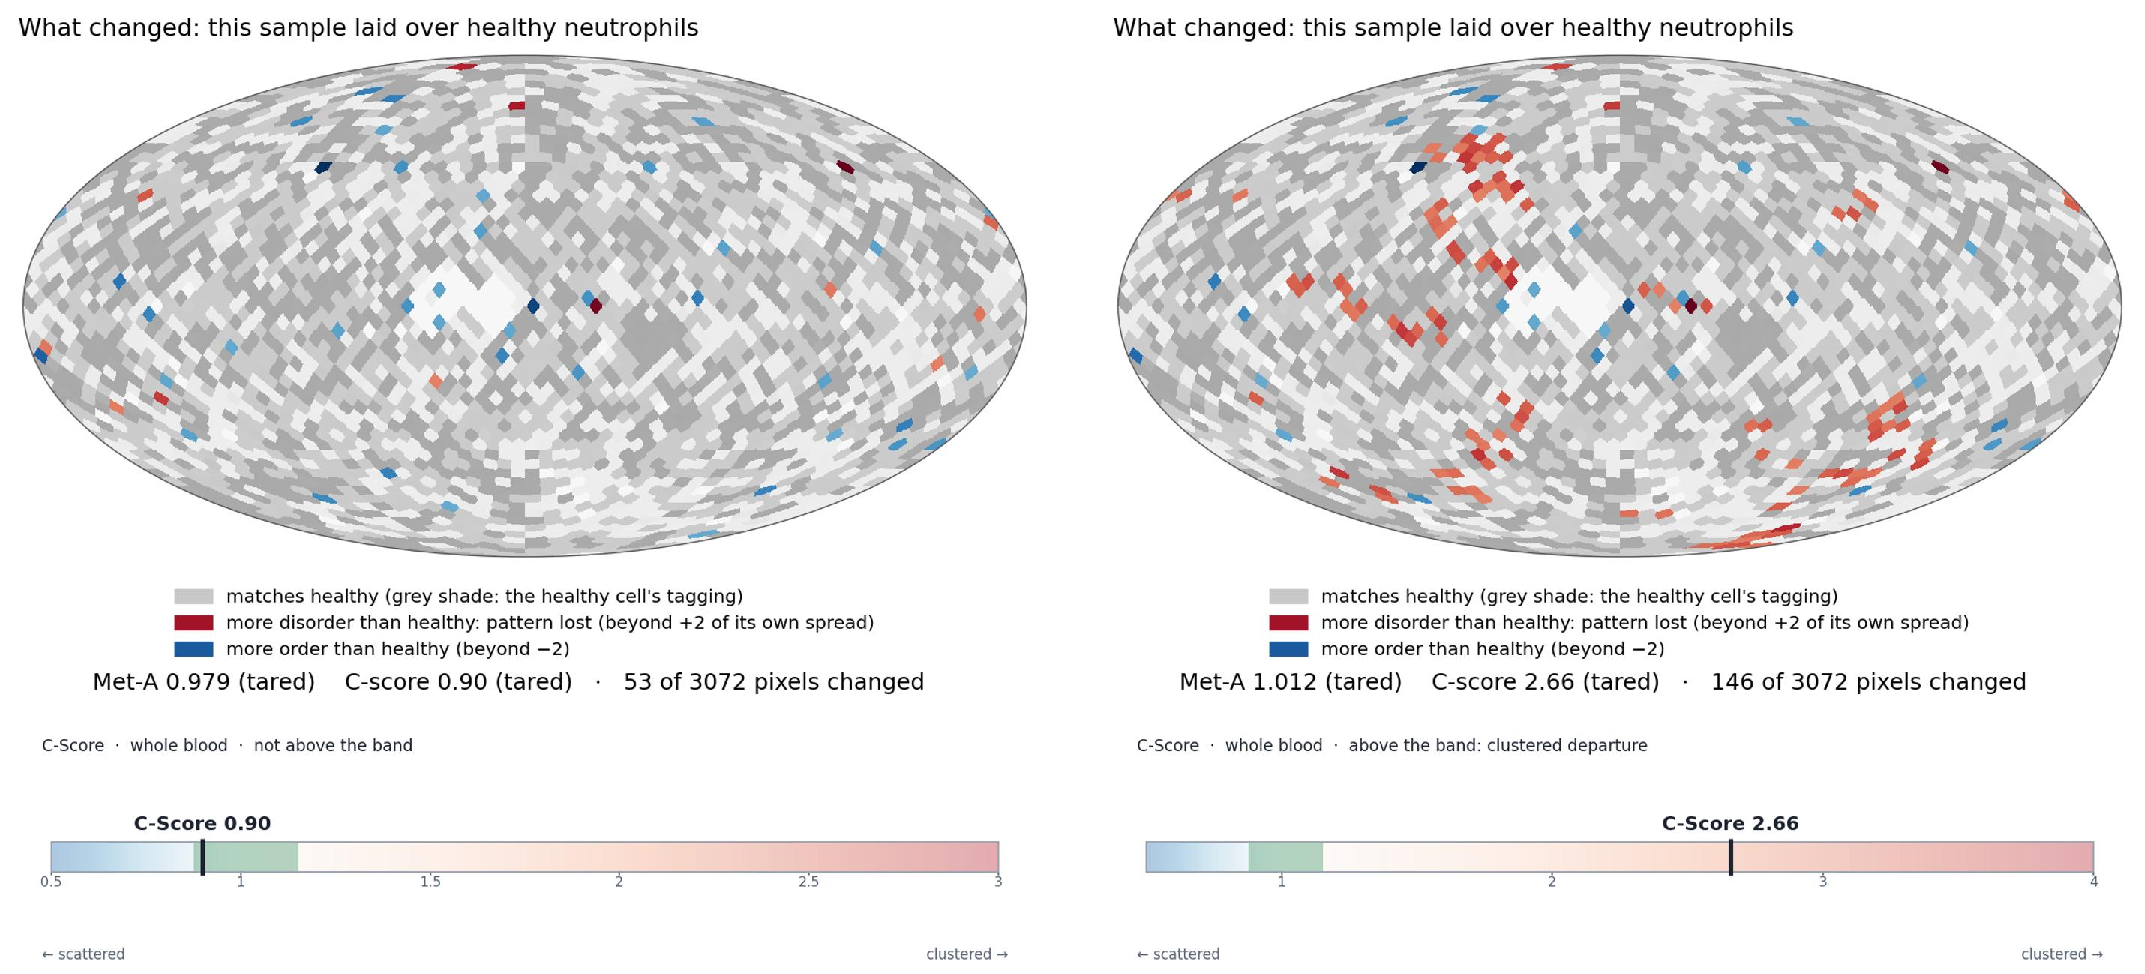
\includegraphics[width=\textwidth]{figures/part6/fig_p6_walk_overlays.pdf}
\caption{The report's sky and C-score bar for a real healthy whole-blood array (left; GSE235717, GSM7508429) and for the same array with a known
clustered change planted into it (right). Grey is where the sample matches healthy neutrophils from IAM-Atlas v2.1; color marks only departures
beyond twice the sample's own spread (red: more disordered than healthy; blue: more ordered). Left: 53 of 3,072 pixels, scattered, $C_{\rm rel}=0.90$.
Right: 146 pixels in streaks, $C_{\rm rel}=2.66$, above the band. Both from the chain's own reports. \measured}\label{fig:walk_overlays}
\end{figure}

\section{The same array, with a known change planted}

To show what the report looks like when the C-score reads above its band, the same array was given a known change, by the C-score's own positive
control rule (Chapter~\ref{ch:cscore}): 10\,\% of its sites, in 20 runs along the genome, each moved 10\,\% of the way toward a coin-toss
methylation of 0.5. The report prints at the top of every view that this is a planted example, not a clinical result.

The C-score reads $C = 2.87$, and $C_{\rm rel} = 2.66$ against the same references: \emph{above the band: clustered departure}, and the report raises
its clustered-departure flag. The sky shows why (Figure~\ref{fig:walk_overlays}, right): 146 pixels, in streaks that follow the genome. Met-A, which
reads the overall level, barely moves: $A_{\rm rel} = 1.012$, still Normal. The two instruments see different things. Met-A asks how far the pattern
has drifted on average; the C-score asks whether the drift is scattered, as aging leaves it, or bunched together along the genome. \measured

Because this sample entered as a table of values rather than as raw files, Stage~0 did not run, and the report says so in its list of cautions. A
reader never has to infer what the chain skipped.

\section{A healthy CD8 T-cell sample, read against itself}

The third sample is whole-genome bisulfite sequencing of healthy blood CD8 T cells (GEO GSM4293895), one of the eight samples of IAM-A's sealed
commissioning test (Chapter~\ref{ch:iama}). It was read from its alignment through the same one command.

IAM-A needs no reference specimen. It counts every qualifying molecule's held error, $\varepsilon = 0.04405$, and the sample's own loose share,
$L = 0.238$; the self-reference line predicts the held error a healthy sample with that loose share carries, $\varepsilon_{\rm pred}(L) = 0.04850$. The
reading is their ratio, $A = \varepsilon/\varepsilon_{\rm pred} = 0.908$, inside IAM-A's Normal band (0.779--1.055): \emph{Normal}. The one command
reproduced the commissioning test's reading of this sample to the last digit. \measured

\begin{figure}[htbp]\centering
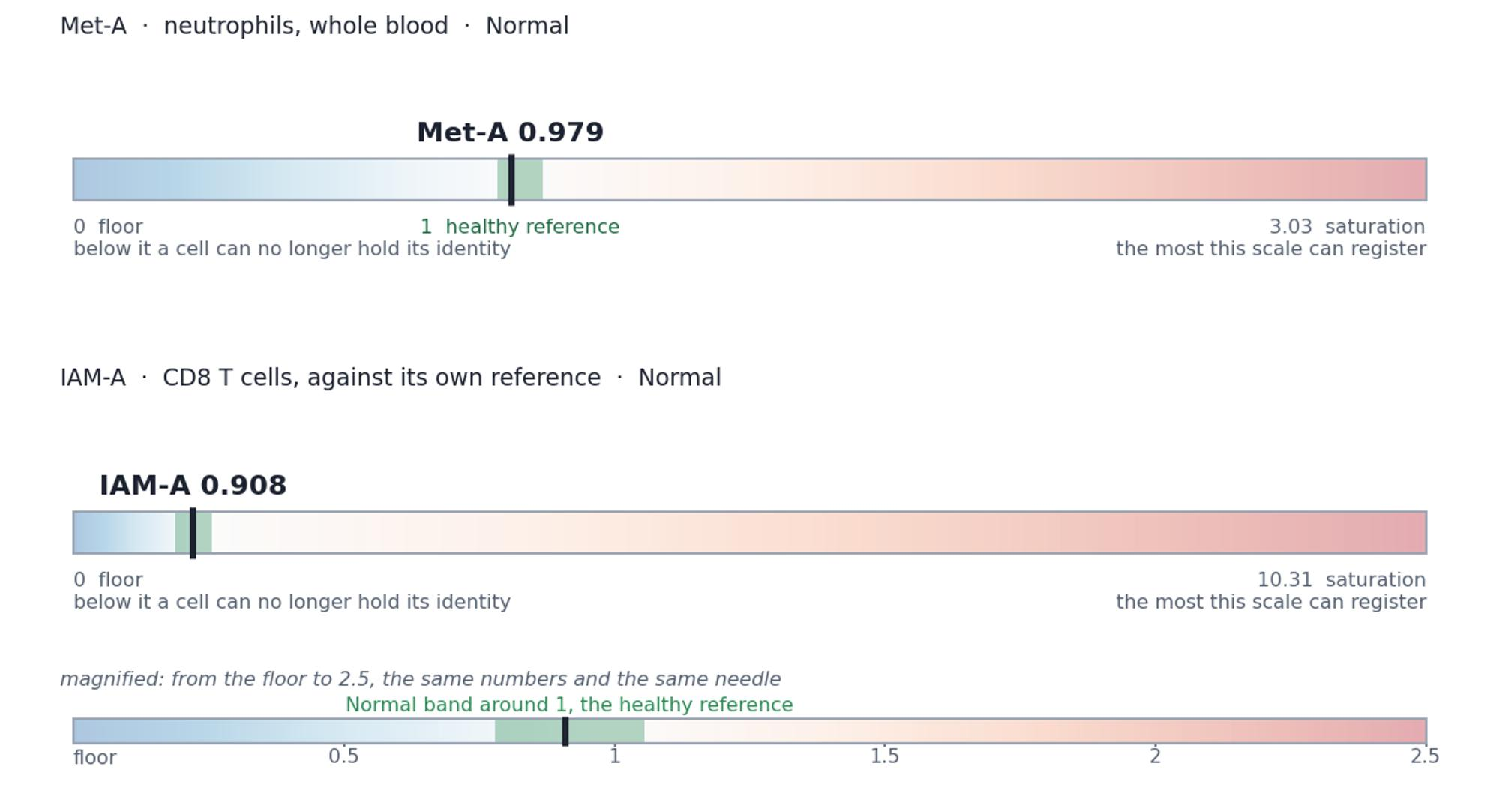
\includegraphics[width=\textwidth]{figures/part6/fig_p6_walk_gauges.pdf}
\caption{The report's gauges. Top: Met-A for the healthy whole-blood array, 0 (the floor, below which a cell can no longer hold its identity),
1 (the healthy reference) and saturation 3.03; tared reading 0.979, Normal. Bottom: IAM-A for the healthy CD8 T-cell sample, 0.908, Normal, on a gauge
whose saturation end is the sample's own ($0.5/\varepsilon_{\rm pred}(L) = 10.31$). Because healthy sits close to the floor on that scale, a magnified
strip under the bar shows the band. \measured}\label{fig:walk_gauges}
\end{figure}

\section{What each view shows}

The Researcher view opens with a table, one line per instrument with its reading, state and status, then \emph{AstroGenetics: the physics behind
each reading}, which gives each reading in bits between its floor and its saturation, then the cell shares, each instrument's section, the sky, and
at the end the technical record of every stage. The Plain view shows the gauges with one plain sentence for each, and the sky. Both views and both
PDFs are built from the same rows, so they cannot disagree.

\section{What these reports show about the chain}

Three things, each on real data. One command reads a raw array or an alignment and writes the full report, with nothing done by hand. Every
reading carries its own reference: the same-run healthy arrays for Met-A and the C-score, and the sample's own loose share for IAM-A. And the chain
says what it did and did not do: a noise index above range, a stage skipped, a cell type outside a commissioned scope are each printed where the
reader sees them.
